
\chapter{Existing Work}
\label{Chap:Lit}

\section{Lighting}

\subsection{Introduction}

Many people do not realise how much time they spend in un-natural lighting conditions. In 2001, a study published in \textit{Nature} magazine found that the average American spends more than three quarters of their time inside \citep{klepeisNationalHumanActivity2001}. More recent studies have put this number as high as 90\% \citep{opiniumBritsSpend902018}, and when most buildings do not get adequate sunlight in the day, the time spent under man-made light sources can be significant. Furthermore, after dark, almost all buildings are lit artificially, very few people around the world do not spend their nights in lit environments.

\citet{falchiNewWorldAtlas2016} found that 86\% of the worlds population, and 99\% of the US and European population live under ``light polluted'' skies. The world uses so much light, that one third of humanity, 60\% of Europeans, and 80\% of North Americans cannot see the Milky Way. 

\subsection{History}

It wasn't always this way. For only the most recent 1.5 million years - a blink of the evolutionary eye - have humans been able to harness the power of fire to extend the usable time of day \citep{gowlettEarliestFireAfrica2013}. It is important to note, however, that fire does not try to emulate daylight; fires used after dark were used for cooking and as a social space \citep{gowlettDiscoveryFireHumans2016}.

It was not until Humphrey Davy and Michael Faraday's contributions to science allowed Davy to produce the first functional electric light: the arc lamp \citep{knightHumphryDavyScience1998}. Since that fateful day, humans' relationship with night has grown increasingly distant. In 1878, Swan presented the first  incandescent lamp, patented by Edison in 1880 (though it is believed that others were developing this technology concurrently) %\citep{montoyaIndoorLightingTechniques2017}
. These bulbs are very inefficient; the peak wavelength is determined by the temperature of the gas in the bulb. In order for visible emission to occur, very high temperatures must be achieved - and still the majority of the light will be infra-red (IR) and not visible to the human eye \citep{montoyaIndoorLightingTechniques2017}.

The next widely adopted innovation was discharge lamps such as sodium lamps and fluorescent tubes, as many Correlated Colour Temperatures (CCTs) could be achieved. Compact Fluorescent Tubes (CFTs) could directly replace Incandescent bulbs using the same fittings.

While LEDs gained widespread popularity in the early $21^{st}$ century \citep{matsumotoMeasuringHouseholdAbility2020}, the first visible light LED was produced back in 1962 by Nick Holonyak \citep{holonyakCOHERENTVISIBLELIGHT1962}, based on the even earlier LEDs of Oleg Losev from 1927 \citep{zheludevLifeTimesLED2007}. It wasn't until 1995 that a non-red LED was produced, solving the issue of monochromasity of LED technology (it was blue) \citep{nakamuraInGaNAlGaNBlue1995}.

Once white LEDs could be produced, it led to the ``Third Revolution'' of indoor lighting \citep{montoyaIndoorLightingTechniques2017}, and now LEDs are ubiquitous in modern life. New LED technology continues to be developed, such as the Organic LED (OLED), which are cheaper and offer better colour rendition. OLED technology has only recently been applied to indoor lighting \citep{phelanOLEDLightingHits2018}, although there are some promising developments in the field \citep{benderSolidStateLightingConcise2015}. However there is still some way to go before OLEDs replace LEDs in artificial lighting technology.

\subsection{Energy Consumption and Environmental Considerations}
\label{sec:Energy}

Incandescent bulbs are not efficient. in fact, they're banned from being sold in the EU because they're so inefficient \citep{euDirective2012272012}. However, this doesn't mean they're all bad, they actually have many benefits; firstly, they produce light much more similar to firelight than modern lighting/ they are also not hazardous, somethin g which cannot be said for fluorescents and LEDs, which also require higher resource depletion to create \citep{limPotentialEnvironmentalImpacts2013}. But LEDs use 85\% less energy and last 50 times longer than incandescents \citep{mottierLEDLightingApplications2010}. This is significant when considering that 20-40\% of most buildings power consumption is from lighting alone \citep{perez-lombardReviewBuildingsEnergy2008}, accounting for as much as 10\% of all power consumed in Europe \citep{bertoldiEnergyEfficiencyStatus2012}. Considering  this, and that LEDs can theoretically convert 100\% of electrical energy to visable light (thermal regulation is key) \citep{jordanChallengesLEDPackaging2012}, it is clear why the wide scale adoption of LED technology has been so rapid \citep{matsumotoMeasuringHouseholdAbility2020}.



\section{Circadian Rhythms}
\label{sec:Circadian}

\subsection{What is the Circadian Rhythm?}

In 1729, the French scientissst Jean-Jacques d'Ortous de Mairan	used plants kept completely in the dark to determine that their diurnal cycles were not caused by external light stimulus, but rather were regulated by some endogenous clock \citep{demairanObservationBotanique1729}. 

\begin{figure}
	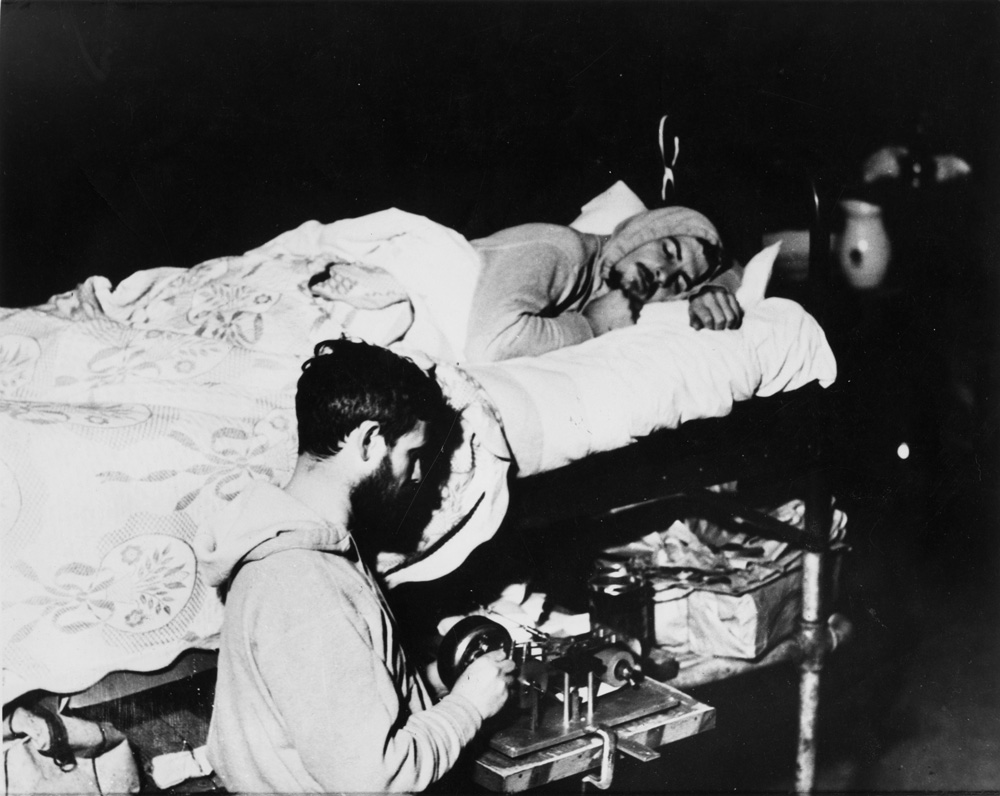
\includegraphics[width=0.5\textwidth]{Images/KleitmanCave}
	\caption{Nathaniel Kleitman (foreground), donning an impressive beard, measures the sleep of  Bruce Richardson \citep{universityofchicagophotographicarchiveKleitmanNathanielPhotographic}.}
	\label{Fig:Cave}
\end{figure}

Amazingly, it wasn't until 1938 that someone repeated this experiment on humans. Dr. Nathaniel Kleitman was a professor of of Physiology at University of Chicago who was later to discover Rapid-Eye Movement (REM) sleep; he is known as the father of sleep research. Together with his PhD student, Bruce Richardson, and a pair of metal beds, they descended into Mammoth Cave in Kentucky for 32 days without any natural lighting stimuli. They found that their sleep-wake cycle did not descend into sporadic bouts of sleep, but rather stayed at a periodic length of around 26 hours, undeniably longer than the 24 hour day. This showed that humans have an internal time-keeping system that lasts about (\textit{circa}) one day (\textit{dian}); they named it the circadian rhythm \citep{kleitmanSleepWakefulness1987}.

\citet{siffreTime1964} repeated this experiment, delving, himself, into a cavern for 2 months, and discovered much the same results. Meanwhile, \citet{vonaschoffSpontanperiodikMenschenBei1962} kept participants in a sealed cellar for 8-19 days, also discovering a circadian rhythm of over 25 hours.

As circadian rhythms are not 24 hours long, they need to be synchronised daily, and thus must rely on a periodic stimulus to entrain them. There were 5 factors that were thought could contribute to this entrainment of the circadian rhythm, as shown in Table \ref{Tab:Factors}.

\begin{table}
\caption{The 5 potential factors for circadian entrainment \citep{czeislerEntrainmentHumanOrcadian1981}}
\label{Tab:Factors}
\begin{tabular}{l l}
\hline
 & \textit{Factor} \\
\textbf{I.}& Knowledge of time of day \\
\textbf{II.}& Light Dark cycle \\
\textbf{III.}& Social Contacts \\
\textbf{IV.}& Timing of food availability \\
\textbf{V.}& Scheduling of bed rest and activity \\
\hline
\end{tabular}
\end{table}


%It was originally thought that the light-dark (LD) cycle (Factor \textbf{II}) was too weak to entrain the circadian rhythms of humans, and that social cues (Factor \textbf{III}) were relied upon \citep{aschoffHumanCircadianRhythms1971}. 

Factor \textbf{I} (knowledge of time) was shown to be insignificant \citep{millsCircadianRhythmsThree1964}. Factor \textbf{II} (light-dark cycles) is the most powerful in many animals and plants, but \citet{aschoffHumanCircadianRhythms1971} concluded that this effect was too weak in humans, and that factor \textbf{III} (social cues) must be our central zeitgerber. 

However, when inspecting the facilities used for these experiments, \citet{czeislerEntrainmentHumanOrcadian1981} realised that the researchers ``\textit{permitted the subjects to use kitchen, bathroom, bedside and desk lamps as sources of self-selected light during the `dark' phase of each cycle}'', prompting a reassessment of the role of light in the entrainment of human circadian rhythms in which he found that light-dark cycles have a ``\textit{direct synchronising effect}'' on human circadian rhythms. They then went on to publish the landmark study titled \textit{Bright light resets the human circadian pacemaker independent of the timing of the sleep-wake cycle} \citep{czeislerBrightLightResets1986}.

\subsection{Melatonin and Melanopsin}

The circadian rhythm is controlled by a part of the brain called the Hyperthalimus \citep{stephanCircadianRhythmsDrinking1972}. Specifically, in the Suprachiasmatic Nucleus (SCN), located above the optic nerve \citep{welshIndividualNeuronsDissociated1995}. The SCN sends signals to the pineal gland \citep{cassoneMelatoninRoleVertebrate1998, borjiginPINEALGLANDMELATONIN1999} which is responsible for the production and regulation of melatonin.\footnote{
There is much intrigue and mystery around the pineal gland, with many believing that it is where conciousness is generated in the brain \citep{bobMelatoninConsciousnessTraumatic2008}. Ren\'e Descartes referred to the pineal gland as the ``seat of the soul'' \citep{lokhorstDescartesPinealGland2020}.
}

Melatonin is known as the sleep hormone, or to some: the ``chemical expression of darkness'' \citep{reiterMelatoninChemicalExpression1991}, and builds up throughout the evening and is essential for sleep onset \citep{arendtImportanceRelevanceMelatonin2003}.

In 2000, a novel Opsin was found in the human eye \citep{provencioNovelHumanOpsin2000}. An opsin is a light-sensitive protein that exists in the visual cells in the eye and is what converts the energy from photons of light into electrical signals that are sent to the brain \citep{terakitaOpsins2005}. It was soon discovered that the action spectrum of this new opsin, malanopsin, did not match any of the action spectra of the known visual cells (rods and cones), implying there was a new cell that we were not yet aware of \citep{thapanActionSpectrumMelatonin2001}.\footnote{
Interestingly, melanopsiin has been found to be much more similar to invertebrate opsins than they are to visual mammalian opsins \citep{provencioMelanopsinOpsinMelanophores1998}. This, as well as the fact almost all animals produce melatonin, shows it is a truly ancient part of our biology \citep{daviesEvolutionFunctionMelanopsin2014}.
} 
This cell was found to be the intrinsically photosensitive Retinal Ganglion Cell (ipRGC) \citep{bersonPhototransductionRetinalGanglion2002}, the signals from which are what keeps the SCN entrained, but to not contribute to concious vision \citep{bersonPhototransductionGanglioncellPhotoreceptors2007}. This explains why some blind people have circadian rhythms that can be entrained with light, as discussed in the review by \citet{allenCircadianRhythmsBlind2019}.

\subsection{Blue Light}

It has been established that light is of great significance in circadian regulation, and that ``moderate illumination'' of around 500 lux \citep{laaksoOnehourExposureModerate1993}, or even ``room light'' of less than 200 lux \citep{gooleyExposureRoomLight2011} can cause a phase shift in the circadian rhythm. Furthermore, due to the action spectrum of the ipRGCs, blue light causes as much larger effect than longer-wavelength light \citep{lockleyHighSensitivityHuman2003}.

The effect of blue light is so potent, that even one second pulses of blue light through closed eyelids are enough to suppress melatonin production \citep{figueiroTrainBlueLight2013}. 

There are a few existing solutions attempting to tackle this problem. For example, the use of amber glasses can filter out blue wavelengths before they reach the retina, and have been shown to improve sleep when worn in the evenings \citep{kimberlyAmberLensesBlock2009}.






\section{Health Implications}
\label{Sec:Health}


In a meta analysis, \citet{sanchez-barceloClinicalUsesMelatonin2010} discuss the potential effects of melatonin in a host of situations, including \textit{``ocular diseases, blood diseases, gastrointestinal tract diseases, cardiovascular diseases, diabetes, rheumatoid arthritis, fibromyalgia, chronic fatigue syndrome, infectious diseases, neurological diseases, sleep disturbances, aging and depression [as well as being] used as a complementary treatment in anaesthesia, hemodialysis, in vitro fertilization and neonatal care''}.

\subsection{Cancer}

We've known for a long time that total visual blindness is protective against many types of cancer \citep{hahnProfoundBilateralBlindness1991, feychtingReducedCancerIncidence1998, flynn-evansTotalVisualBlindness2009}. It was also observed in many studies that flight attendants were more likely to develop breast cancer, as summed up in the meta analysis by \citet{tokumaruIncidenceCancerFemale2006}. This effect was also observed in night-shift workers, shown in two large reviews of the existing evidence \citep{kolstadNightshiftWorkRisk2008, stevensLightatnightCircadianDisruption2009}. It is also known that the circadian rhythm has a cancer-suppressing effect \citep{fuCircadianClockPacemaker2003} and that circadian disruption is a promoting factor for lung cancer \citep{papagiannakopoulosCircadianRhythmDisruption2016}. An extensive meta analysis even found that chemotherapy toxicity is correlated to when it is taken, leading to the entire field of chronotherapy \citep{focanCircadianRhythmsCancer1995, dallmannChronopharmacologyNewInsights2014}.

The correlation of circadian regulation and cancer is so well recognised, that even the WHO classes night-shift work as a class 2A carcinogen \citep{whoBreastCancerConundrum2013}. However, even those not engaging in abnormal working hours may have an increased risk; \citet{stevensBreastCancerCircadian2014} blames electric lighting directly as the cause of breast cancer being the leading cause of cancer death among women worldwide.


\subsection{Diabetes}

Although 415 million people worldwide live with Type II Diabetes, it is a preventable and reversible disease \citep{fungDiabetesCodePrevent2018}. Type II diabetes is a lifestyle disease, mostly caused by diet, whereby insulin resistance is built up such that blood sugar can no longer be absorbed by cells. A contributing factor to this is melatonin, which has been shown to aid blood glucose homoeostasis \citep{bouatia-najiVariantMTNR1BAssociated2009}. Melatonin receptors influence fasting glucose levels \citep{prokopenkoVariantsMTNR1BInfluence2009} and when completely removed, can even induce insulin resistance \citep{contreras-alcantaraRemovalMelatoninReceptor2010}.

Another study found that social jetlag - the jetlag-like effect of inconsistent waking times, ie. waking up later at the weekend - is a risk factor for obesity, itself the largest risk factor for Type II Diabetes and a host of other health issues \citep{roennebergSocialJetlagObesity2012}

\subsection{Seasonal Affective Disorder}

Seasonal Affective Disorder (SAD) is caused by a lack of light in the wither months when the sun is lower and takes a shorter path across the sky \citep{eastmanNaturalSummerWinter1990}. It has been long considered a fact that bright light helps alleviate the symptoms of SAD \citep{magnussonTreatmentSeasonalAffective1991, leeSpectralPropertiesPhototherapy1997,eastmanBrightLightTreatment1998}, but this has actually been quite a controversial topic, with others claiming that the placebos in these studies were not adequate, and such that the anti-depressant effect can be attributed to placebo effect \citep{eastman26ComparisonTwo1993}. A comprehensive meta-analysis found that only 13\% of studies published between 1975 and 2003 were adequate in their methods \citep{goldenEfficacyLightTherapy2005}. It also highlihgted the importance of dawn simulation, which beats out both bright-light and placebo effects significantly \citet{averyDawnSimulationBright2001}.


\section{Cortisol and Attentiveness}
\label{Sec:Cortisol}

Melatonin is essential for sleep, building throughout the evening and peaking in the middle of the night. Similarly, Cortisol - produced in the adrenal gland - helps us wake up, and peaks around mid-morning. This is known as the Cortisol Awakening Response (CAR) and is, of course, also regulated by the circadian rhythm \citep{friesCortisolAwakeningResponse2009}.

Cortisol is the hormone of wakefulness and alertness and such it has been shown that a higher spike in morning cortisol is correlated with better cognitive performance \citep{evansDiurnalCortisolCycle2011}, and general daytime cortisol improves alertness \citep{chapototCortisolSecretionRelated1998}. It is clear, then, that we want to maximise the CAR, which can be done through exposure to short-wavelength (blue) light after awakening \citep{figueiroShortWavelengthLightEnhances2012}. Dawn-simulation has also been shown to improve the CAR - more so than just blue light - as well as improving melatonin regulation, increasing well-being, mood and cognitive performance \citep{gabelEffectsArtificialDawn2013}.

It is also well documented that cortisol is a large contributing factor to mood disorders, especially bipolar disorder \citep{youngCortisolMoodDisorders2004}. A study by \citet{sitLightTherapyBipolar2007} found that \textit{``Women with bipolar illness are highly sensitive to morning bright light treatment''}, following this up a decade later with a double-blind placebo controlled trial that found that 68.2\% of the bright light participants had their bipolar disorder go into remission, compared with only 22.2\% in the placebo group \citep{sitAdjunctiveBrightLight2017}.

\section{Mood and Lighting}

Lighting arrangements affect how we percieve spaces \citep{durakImpactLightingArrangements2007}, with the general finding being that daylight-style LEDs are the most comfortable during daytime hours \citep{cajochenEffectDaylightLED2019}. It is also known that red ambient lighting is more relaxing than blue \citep{lauferPsychophysiologicalEffectsColoured2009}, and that blue causes more stimulation that red \citep{schweitzerInvestigationGenderAgerelated2016}. Pulsating orange light has also been shown to be even more relaxing \citep{wanInfluenceLightingColor2012}, it seems as though this could have a link to the fact it is a closer approximation to firelight.

Full-spectrum lighting has been thought to improve cognitive performance and mood states \citep{berryWorkEfficiencyMood1984}, however this is somewhat controversial and likely to be a placebo effect \citep{veitchDemandCharacteristicsFull1991}.

\begin{figure}[t]
\centering
\LARGE
\textbf{``Light affects our sleep more powerfully than any drug''}

\citep{czeislerPerspectiveCastingLight2013}
\end{figure}


\section{Summary of Literature}
\label{sec:LitSummary}

Over the past 150 years, electric lighting has gone from a pipe-dream to an everyday necessity, increasing the length of the productive day. 

Alongside these developments, circadian science has been driving forward, from observations of the nature of free-running circadian rhythms to the discovery that light has profound affects upon it. Blue light's effect is especially powerful and is becoming more and more ubiquitous as our technology advances. As \citet{czeislerPerspectiveCastingLight2013} says in his landmark perspective piece entitled \textit{Casting the Light on Sleep Deficiency: ``Technology has effectively decoupled us from the natural 24-hour day to which our bodies evolved''}. 

This decoupling is dangerous for many aspects of our health. Not only is sleep important for all aspects of health and well-being, melatonin itself has a promising effect on many diseases including type II diabetes, SAD, cancer, and many others. Cortisol, melatonin's sister hormone, is also essential for a healthy life and promotes attentiveness, alertness and cognitive function.

Looking to the past for answers, we see that the output spectra of more outdated technologies such as incandescent bulbs are far more appropriate for evening use than the more modern fluorescent tubes and LEDs. But these older technologies are far less energy efficient, to the point that their sale is banned in the EU. On the other hand, the adoption of more energy efficient technologies should not come at the expense of human health \citep{boyceReviewImpactLight2010} due to excessive blue light exposure - which has also been shown time and again to damage our eyes in excessive quantities \citep{uedaEyeDamageControl2009, kuseDamagePhotoreceptorderivedCells2014, niwanoBlueLightInjures2014, marekBlueLightPhototoxicity2018, nakamuraExposureExcessiveBlue2018}.

Blue light is not all bad, though. Its effects on SAD, bipolar disorder, and cognitive ability show that it is all about giving our body the right light at the right time of day. Some people already strive for this by using blue-light blocking glasses or RGB LED bulbs that can be set to change colour. These technologies are flawed, though: glasses are a hassle to wear and carry around and RGB LEDs only approximate perceived colours by combining red, green and blue, thereby ensuring there is more short-wavelength light that is desirable \citep{gilewskiEcologicalHarmfulnessRGB2018}.

This has led many to believe that an overhaul in the lighting used in the built environment is of paramount importance, with many papers calling for immediate action \citep{webbConsiderationsLightingBuilt2006, boyceReviewImpactLight2010, groseArtificialLightNight2014}.




\section{Existing Solutions}
\label{Lit:solutions}

An analysis of existing solutions was undertaken early in the project to understand what already exists in this field. The products could be generalised into 4 categories:

\subsection{Wake-Up Lights}

Ranging from £20 to £200, these products usually come in the form of an alarm clock with a built in light to wake up the user with a simulated dawn. With many varying features across the models, most contain an FM radio.

These lamps are used as a bedside light and are not appropriate for lighting a whole space. As they are focused on morning light, many use inappropriate spectra to be used before bed.

 While these devices utilise an artificial dawn - shown to have many beneficial effects - there are few studies on these devices themselves.

\subsection{Bulb Replacements}

Various forms of smart-light exist on the market currently, most notably the Philips Hue. this can be set to fade to warmer light in the evenings and brighter light during the day to encourage winding-down and focus respectively. 

However the basis of these are very much visual entertainment, not circadian entrainment. Using RGB LEDs, they are less than ideal for use before bed and need serious modifications to automatically change temperature.

These bulbs are expensive, too.  For a starter kit including the base unit and just 4 bulbs, Philips charge almost £200.

Circadian bulbs also exist. These are fitted to dimmer circuits and change temperature instead of dimming. BIOS lighting have a natural-spectrum bulb that can be used both in day and night. However, these require manual adjustment throughout the day and require dimmer circuits to be installed.

\subsection{Industrial Circadian Lighting}

There are many companies offering bespoke services to fit circadian lighting systems into office spaces and warehouses. However these are very expensive and not applicable for home installation. Furthermore, as they are designed for business environments, many of these solutions do not account for later evening that can aid with sleep onset.

\subsection{Software Based}

Windows, OSX, iOS and Android all now have built in blue light filters that can be turned on to limit the amount of blue light that the screen emits. The intensity and time that it comes on can usually be adjusted by the user. Specialist software such as f.lux can also be used for this purpose but with greater flexibility.

\subsection{Discussion}

All of the devices discussed here have one other feature in common: as they are all LED devices based on providing a visual cue and are not designed based on the evidence in the literature at the forefront (perhaps with industrial solutions as the exception), the spectra of these devices can be questionable.

Also, none of these products are designed to get dim enough to be used late at night. They are all for use leading into the evening, but once the user is in bed, these become insufficient solutions.

\section{Implementation}

The ideas discussed in this chapter were used to inform the requirements specification (Appendix \ref{App:Req}). The output spectra of the lamp will have to be respectful of biological considerations: no light produced within the melanopsin action spectrum during the evening, but high blue light in the morning. Dawn simulation must be achievable on the device to gain many of the benefits.

The existing solutions have shown that the device must be low cost, and fully automated to bridge all of the shortcomings of the current devices. The device should also be simple to install and not require additional technology such as a smartphone.